\chapter{Introducci\'on}


El estudio del Sol ha resultado indispensable para el desarrollo de la humanidad. En la antig\"uedad, por ejemplo, la observaci\'on del Sol permiti\'o al g\'enero humano estimar la duraci\'on de las estaciones del a\~no; lo cual permiti\'o realizar predicciones, entre muchas otras cosas sobre la agricultura y los mejores tiempos para emprender largos viajes. Hoy en d\'ia, el estudio del Sol est\'a indisolublemente relacionado con el progreso de nuestras tecnolog\'ias. Por ejemplo, se puede decir que la actividad del Sol, particularmente de su atm\'osfera tienen una relaci\'on directa con nuestros avances aeroespaciales y en materia de telecomunicaciones.

El estudio de \'este astro resulta importante, pues como ha ocurri\'do con anterioridad, la actividad solar puede incluso llegar a da\~nar infraestructuras en telecomunicaciones, redes el\'ectricas y/o sistemas de geo-posicionamiento global (GPS)\citep{carrington}. Uno de los prominentes rasgos manifestados por la actividad solar son los repentinos y radicales abillantamientos conocidos como r\'fagas solares que son eventos en donde se aceleran cargas el\'ectricas liberando descomunales cantidades de energ\'a de t\'ipicamente de $10^{32}$~ergs en forma radiante, en forma t\'ermica y en forma cin\'etica ~\citep{carrington}. A su vez, las r\'afagas solares usualmente anteceden a fen\'omenos de mayor escala conocidos como Eyecciones de Masa Coronal (EMC), que son desprendimientos de vastas porciones de la atm\'osfera externa del Sol y que se proyectan al medio interplanetario, y que eventualmente arriban a la Tierra causando potenciales desastres naturales y tecnol\'ogicos como los descritos en~\citep{carrington}

Es as\'i como el diagn\'ostico del estado f\'isico de la atm\'osfera solar conlleva a importantes cuestionamientos y avances en la descripci\'on del modo en c\'omo se genera y se transporta energ\'ia a trav\'es de \'esta, principalmente en un estado previo a la gestaci\'on de las r\'afagas solares y EMC (Emisi\'on de Masa Coronal).

Sin embargo, hasta el momento, a la disciplina de la f\'isica solar le ha resultado imposible desarrollar un modelo preciso que prediga el comportamiento de la atm\'osfera solar. Esto se debe a que a\'un no se posee conocimiento del todo certero de la f\'isica ivolucrada. En principio, existe una multitud de trabajos cuyo argumento para las repentinas y radicales variaciones de la atm\'osfera solar, las cuales son causadas por inestabilidades de los campos magn\'eticos preexistentes \citep{chromotemp}, \'esta es una suposici\'on basada en fuertes evidencias observacionales. 

Esta relaci\'on causal ha sido estudiada mediante modelos emp\'iricos que se basan en procesos f\'isicos formulados previamente. El poder de c\'omputo limita la resoluci\'on espacial (y posiblemente temporal) que por lo regular no alcanza el poder de resoluci\'on de instrumentos que actualmente observan el Sol, por lo que los resultados en las simulaciones se presentan como cantidades promediadas en una determinada escala de espacio y tiempo. 

Son dos trabajos los que se realizan en los modelos uno es el de resolver las ecuaciones de la estructura que describen a la atm\'osfera solar y el otro es el de resolver la ecuaci\'on de transporte radiativo a trav\'es de este medio. Los resultados devueltos son distribuciones de temperaturas, densidad y otros par\'ametros f\'isicos  respecto a la coordenada radial, i. e. hablamos de modelos de car\'acter unidimensional y su consistencia est\'a determinada de comprar la emisi\'on o espectro simulado del transporte radiativo con las observaciones. 

La dimensionalidad de un modelo es una aproximaci\'on que est\'a sujeta a la resoluci\'on abordada. Para un modelo unidimensional, la escalas horizontales de resoluci\'on son mayores que las correspondientes escalas verticales, es decir, los cambios en el flujo emergente, en la densidad, temperatura, etc., ocurren en esta direcci\'on ~\citep{Fontenla2006}.

Dado que el conocimiento de algunos procesos f\'isicos est\'a incompleto es necesario emplear valores \emph{ad hoc} de par\'ametros correspondientes para describir algunos efectos en el medio. En la implementaci\'on de un modelo se busca la consistencia f\'isica sobre las escalas espaciales proyectadas para la simulaci\'on por lo que las estructuras finas no son expl\'icitamente abordadas en el an\'alisis ya sea por el poder de c\'omputo o or que la f\'isica involucrada con esas escalas no est\'e completamente entendida.

En resumen, el principal objetivo de el modelado te\'orico es el de entender los procesos f\'isicos b\'asicos mediante un tratamiento consistente, y en segundo reporoducir a detalle las observaciones bajo las simplificaciones asumidas.

Uno de estos modelos semi-emp\'irico toma en cuenta una atm\'osfera hidrost\'atica en cuyo medio se resuelve la ecuaci\'on de transporte radiativo y reproduce la emisi\'on observada con una similitud razonable a la observada. Para ello se consideran dos hip\'otesis; la primera es que el campo magn\'etico no tiene efecto sobre las escalas del flujo convectivo y la segunda es que el modelo es unidimensional. Lo cual resulta en una atm\'osfera plano-paralela estratificada horizontalmente y en equilibrio hidrost\'atico.

Algunos resultados de la aplicaci\'on del modelo semi-emp\'irico hidrost\'atico fueron primeramente publicados por (Smerd, 1950; van de Hulst, 1953; Allen, 1963; Ahmad \& Kundu, 1981; Vernazza, Avrett \& Loeser, 1981(VALC); Fontenla et al. 2006(SRPM305)). En la Figura~\ref{semi_emp}. Se muestran los perfiles unidimensionales de la temperatura y densidad que explican la emisi\'on emergente. Adem\'as de los modelos citados arriba, se muestran las componentes fr\'ia (1000A) y caliente (1008Q) del modelo de Fontenla et al. 2011.


%Este modelo semi-emp\'irico hidrost\'atico explica con buena aproximaci\'on la emisi\'on emergente en el rango visible-UV (Fontenla et al. 2006), sin embargo en el rango mm-IR hay una discordancia entre el espectro simulado y el observado alrededor del posic\'on donde se registra el valor m\'inimo del perfil de la temperatura.


\begin{figure}[h!]
  \centering
  \begin{subfigure}[b]{0.4\linewidth}
    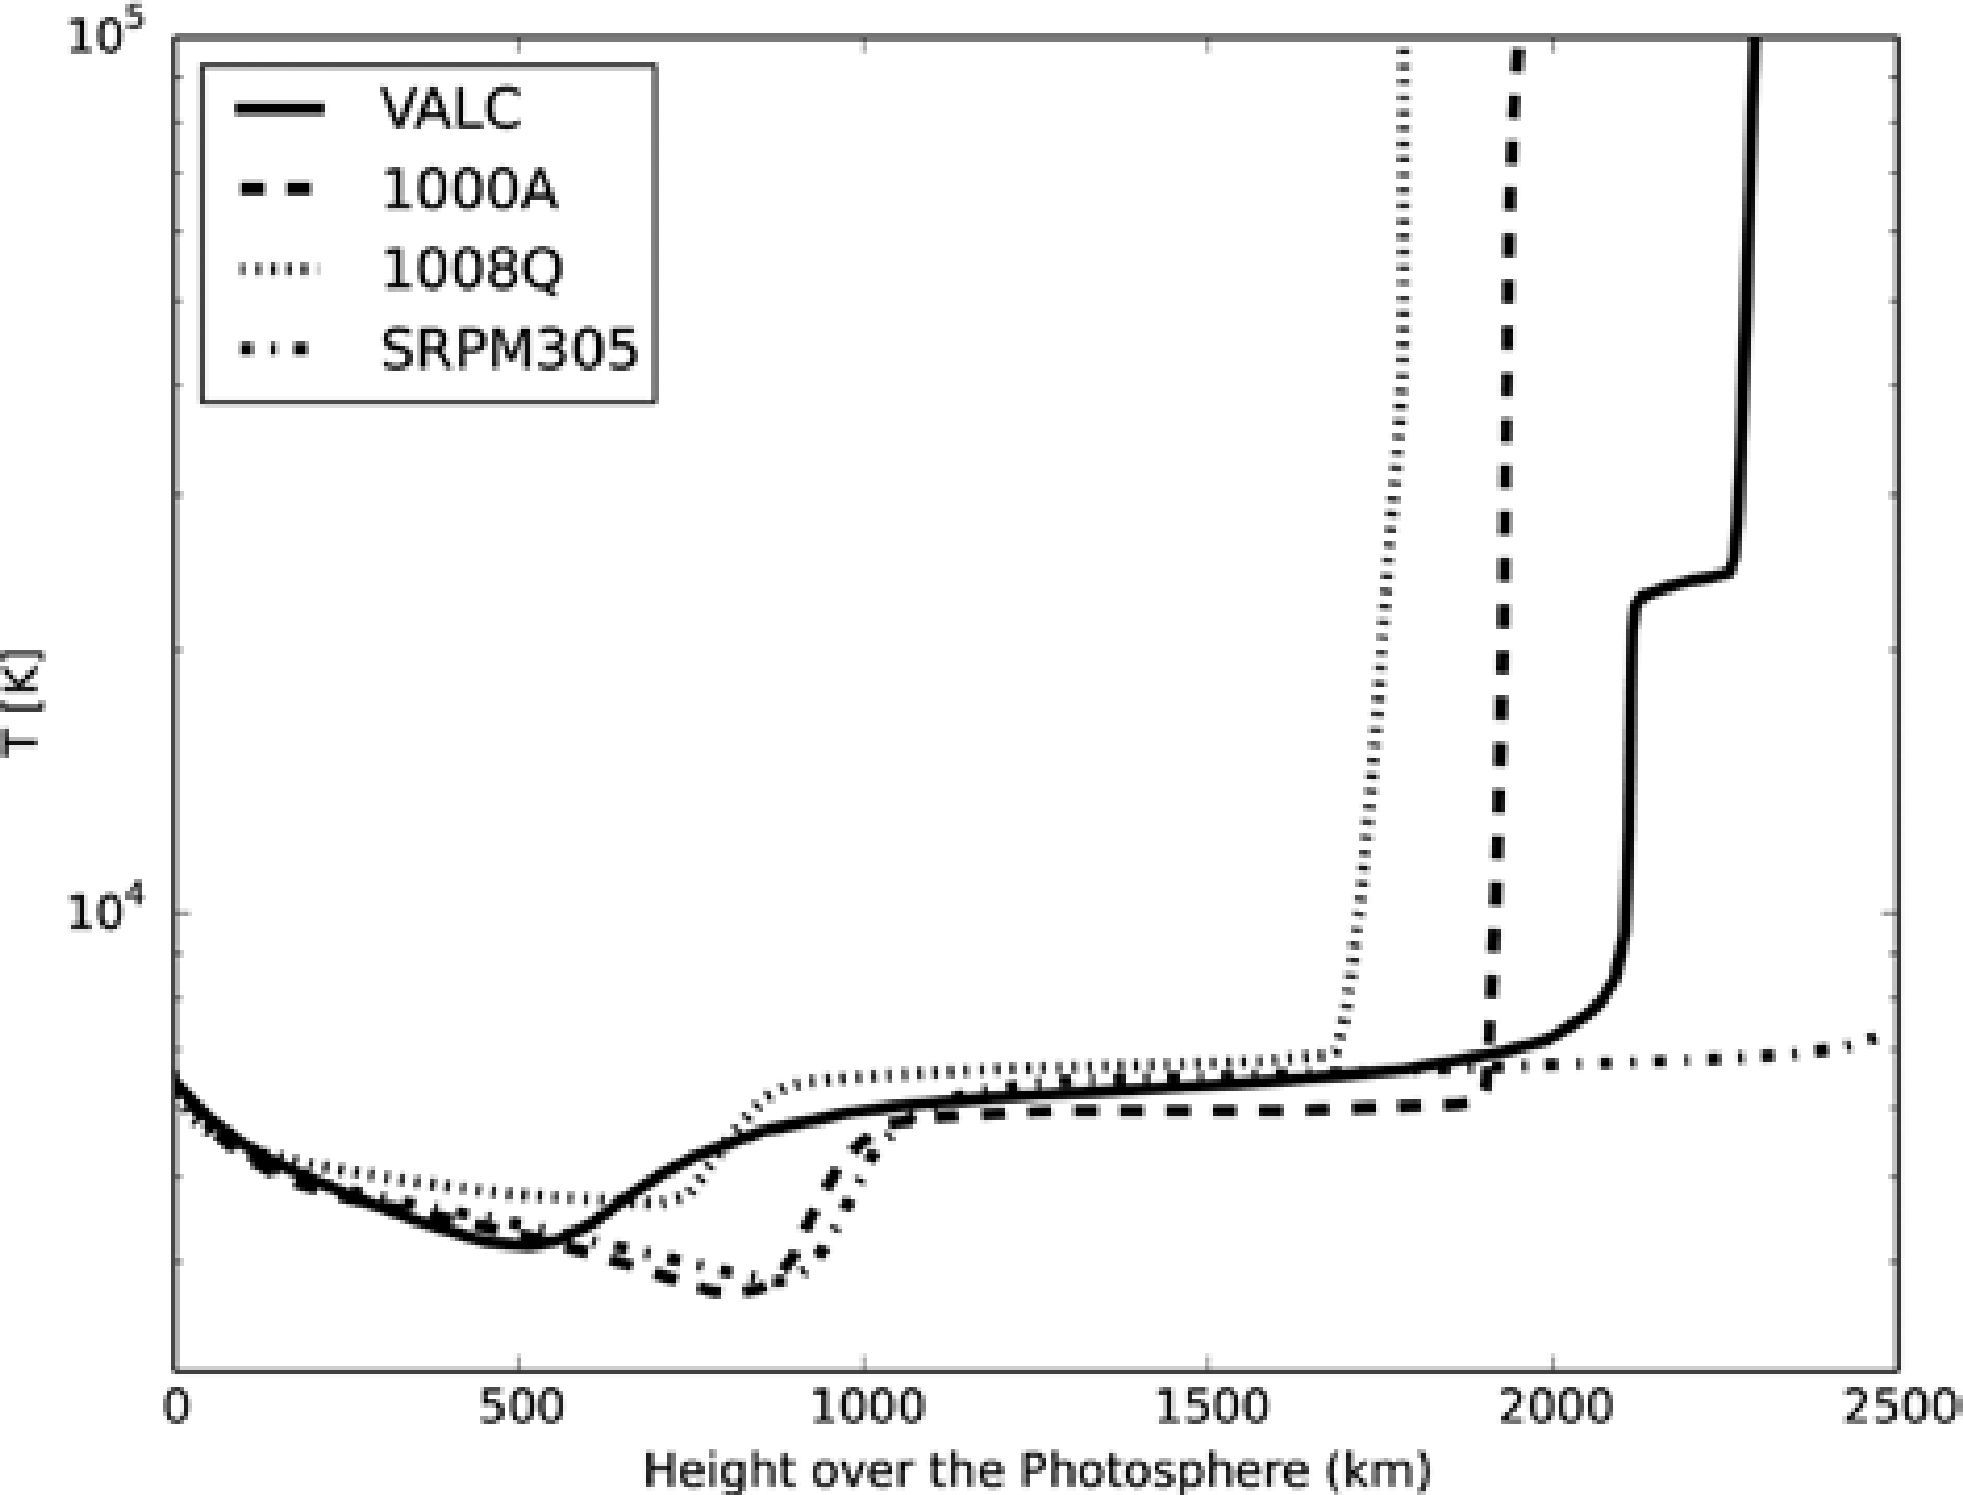
\includegraphics[width=\linewidth]{temperature_profile}
    \caption{Perfil de temperatura}
  \end{subfigure}
  \begin{subfigure}[b]{0.4\linewidth}
    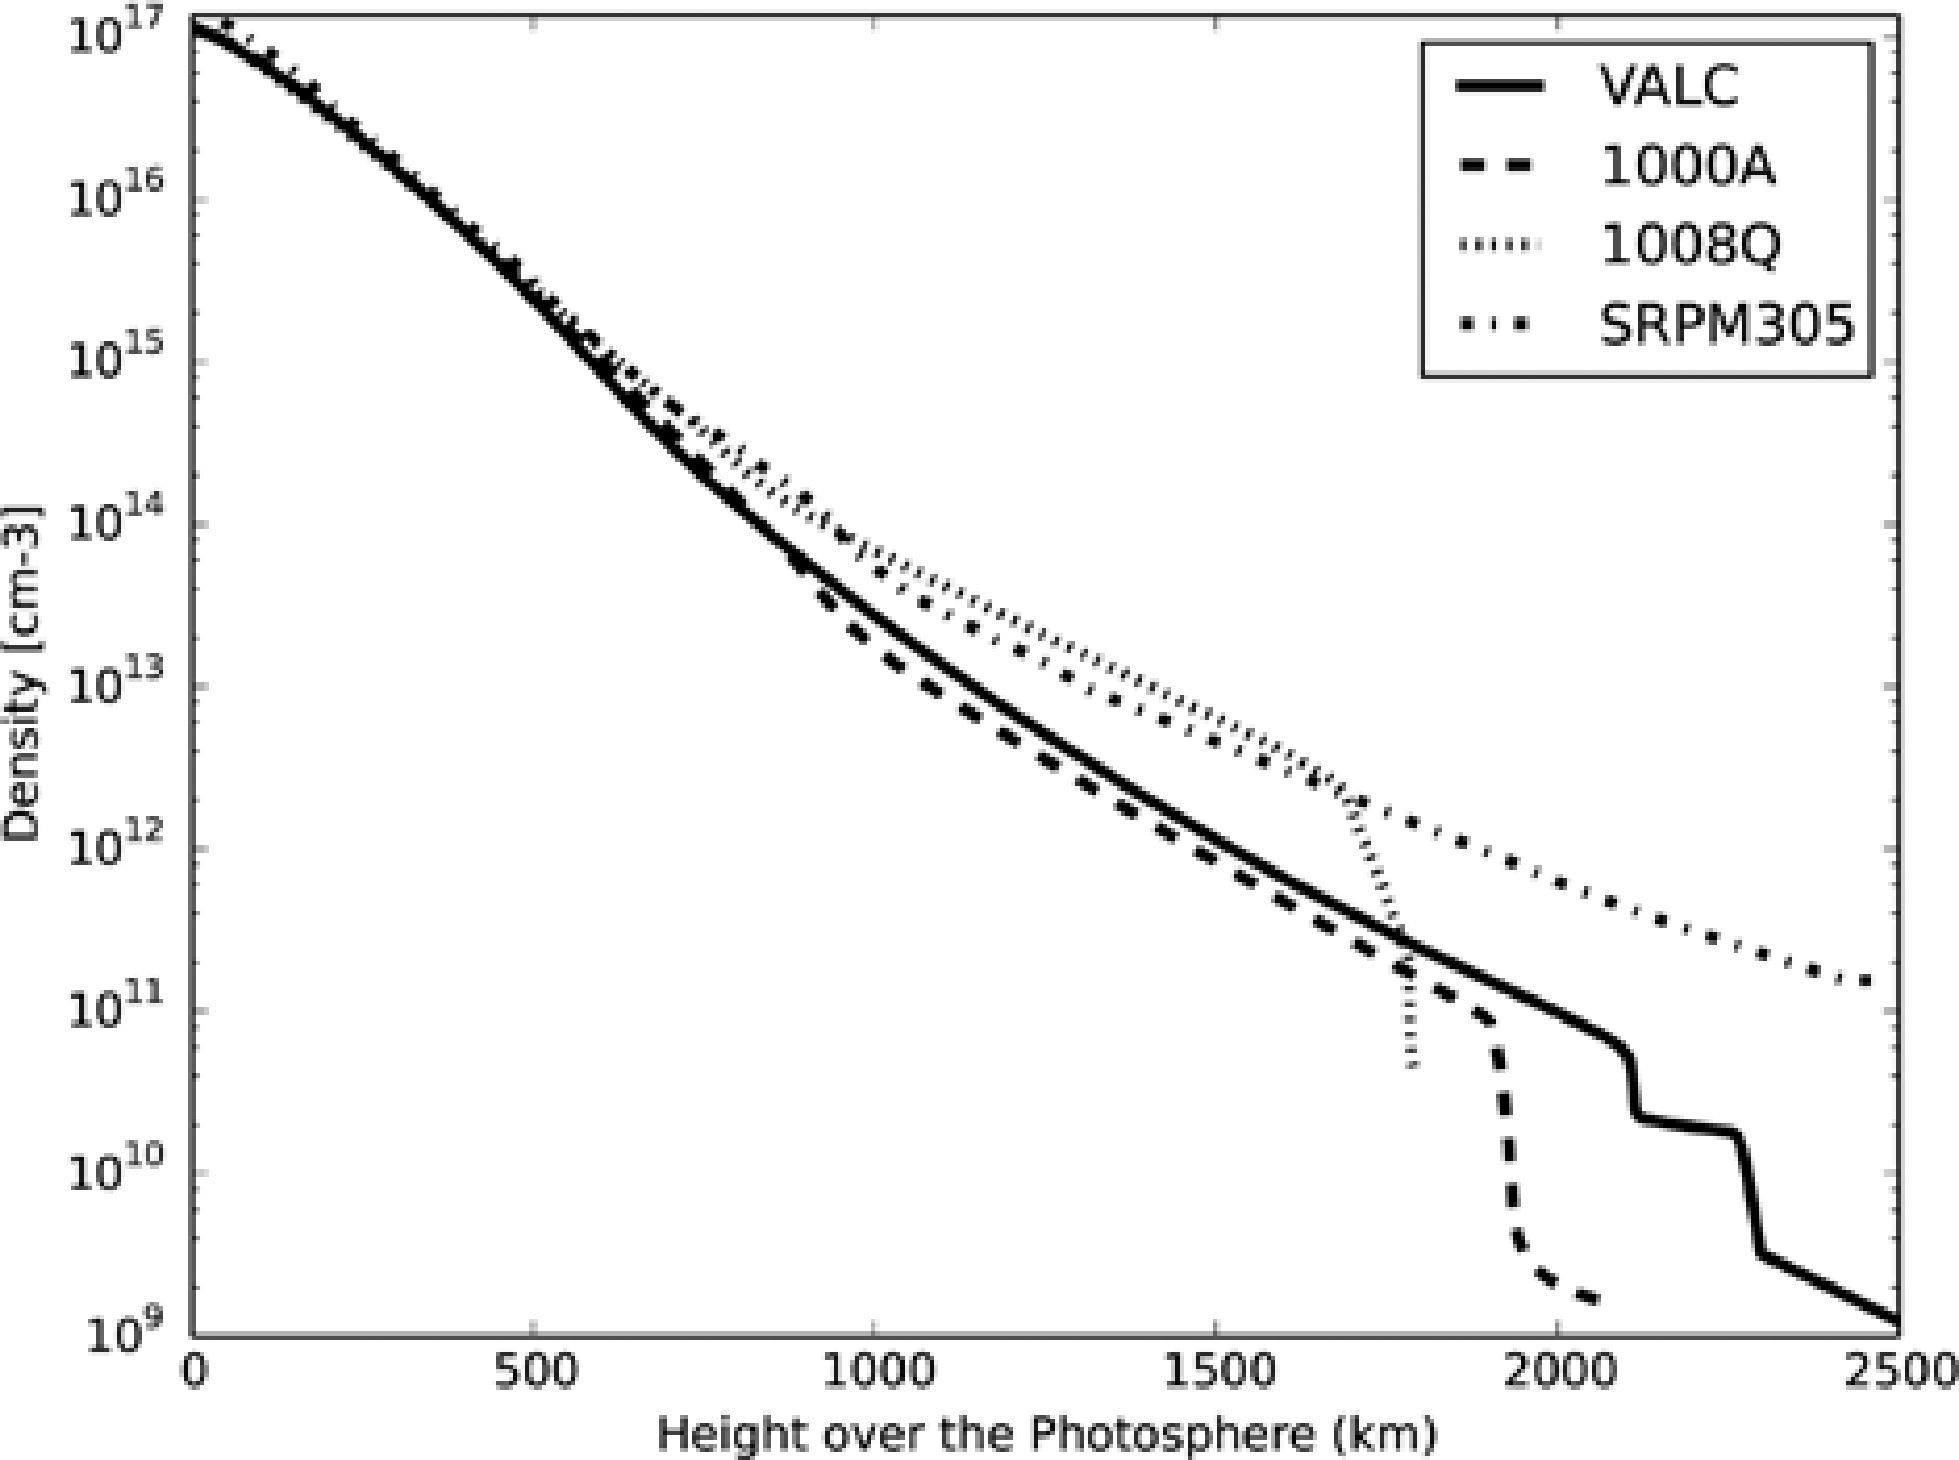
\includegraphics[width=\linewidth]{density_profile}
    \caption{Perfil de densidades}
  \end{subfigure}
  \caption{ (a) Perfiles de temperatura para los modelos VALC, SRPM305, 1000A y 1008Q los cuales muestran un m\'inimo de temperatura entre los 100 y 1000~km de altitud sobre la fot\'osfera. (b) Perfiles exponenciales de densidad que parte desde niveles fotosf\'ericos hasta altitudes alrededor del valot m\'inimo de la temperatura.}
  \label{semi_emp}
\end{figure}




Esta tesis extiende el estado del arte de la f\'isica solar mediante dos principales contribuciones. La primera contribuci\'on reside en proveer evidencia parcial y exploratoria, a trav\'es de una simulaci\'on computacional,  que las variaciones repentinas y radicales de la crom\'osfera se deben al efecto de los campos magn\'eticos de los niveles cromosf\'ericos y coronales. La segunda contribuci\'on consiste en complementar un modelo de simulaci\'on computacional existente para que considere el efecto de los campos magn\'eticos mismos. Con relaci\'on a esta segunda contribuci\'on, se refiere al modelo de simulaci\'on computacional llamado \emph{Pakal}, empleado para diagnosticar la emisi\'on milim\'etrica y submilim\'etrica proveniente de niveles coronales~\citep{2010ApJS..188..437D} con una resoluci\'on espacial comparable con la alcanzada con el instrumental actual.

Este c\'odigo est\'a escrito en C/MPI con licencia GNU/GPL. \emph{Pakal}MPI toma como dato de entrada, el perfil de densidad del Hidr\'ogeno, temperatura y metalicidad; calcula las abundancia en Equilibrio Termodin\'amico  Local (ETL) para 18 \'atomos y las abundancias de H, H$^{-}$ y electrones para fuera de ETL (NETL). Luego, calcula la trayectoria del haz y resuelve las ecuaciones de transferencia radiativa usando integraciones a lo largo de dicha trayectoria en segmentos cuya longitud es controlada por un algoritmo inteligente. La soluci\'on de la ecuaci\'on de transferencia depende de la profundidad \'optica empleando tres distintos mecanismos de absorci\'on/emisi\'on: Bemsstrahlung, H$^{-}$ y Bremsstrahlung inverso. Finalmente la temperatura de brillo la profundiad \'optica y las opacidades se registran en la proyecci\'on radial de cada paso.

Actualmente, el c\'odigo de Pakal realiza sus modelos de simulaci\'on sin considerar el efecto de los campos magn\'eticos en el c\'alculo de la densidad del plasma emisor de la crom\'osfera. Esto ocasiona que sus resultados sobre la densidad no sean del todo precisos en comparaci\'on con las observaciones reales. Mediante la extensi\'on del c\'odigo propuesta en esta tesis, se le posibilita a Pakal la capacidad de considerar el efecto de los campos magn\'eticos. Como resultado, sus aproximaciones a la densidad observada son m\'as precisos. Lo anterior permite robustecer el conocimiento de las variaciones repentinas y radicales observables en la temperatura de la crom\'osfera a partir de par\'ametros de la estructura magn\'etica tridimensional.
